\chapter{Appendices}
For more detailed discussion of methods that doesn't make a key contribution to the main text of the thesis.

\section{Acknowledgements}
The long list of people who helped in some way.


\section{Ethics} \label{sec:ethics}
Everything related to ethics approval, including letter of invitation etc.

There must be a standard form of words for this; reference approval number etc.

\begin{figure}[p]
    \centering
    \frame{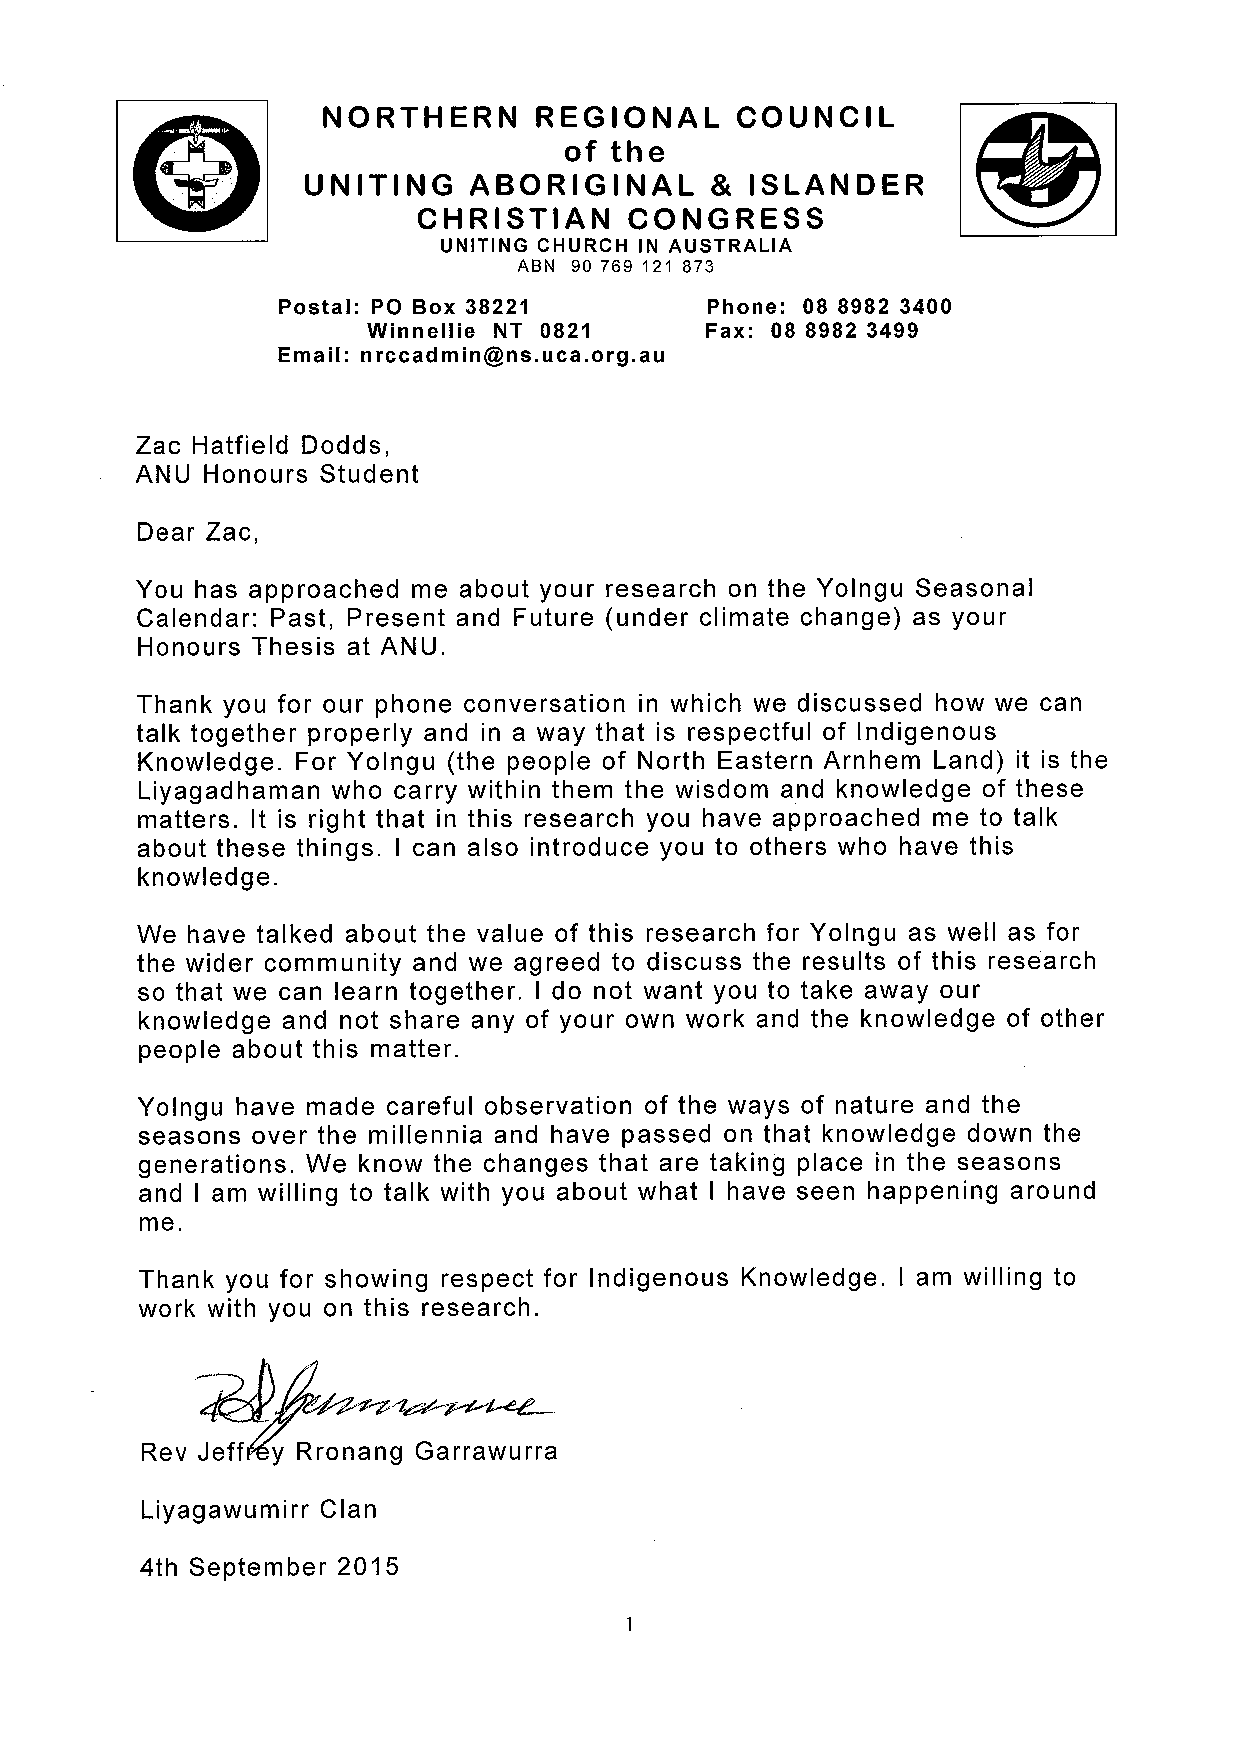
\includegraphics[width=0.9\textwidth]{invitation-letter.pdf}}
    \caption[Letter of invitation for collaborative research]{
        The formal invitation to study Yolngu seasons,
        and share results with both first and second peoples.
        Pre-existing relationships, with Yolngu and non-indigenous people,
        were essential in arranging this collaboration.
        }
    \label{app:invitation-letter}
\end{figure}


\section{Code and Data}
All the code and data I used are included in the supplementary material,
attached as electronic appendices.  Additional copies available on request.

To ensure long-term preservation of the electronic appendices, they
are provided as a .zip archive with the following SHA1 checksum:

da39a3ee5e6b4b0d3255bfef95601890afd80709

(that's the hash of an empty string, as the archive mentioned doesn't exist yet)



\section{Other approaches}
Note that where appropriate items in this section would simply be folded into the main text.
Remaining content is likely to be cut before finalisation,
but it's a useful dumping ground during the drafting process.

-	things I tried which didn't work – eg code ideas, fieldwork attempts, etc.
-	things I didn't try but might work – ie ideas for further study
-	why I didn't try things I thought were a bad idea or waste of time

It would be really interesting to see further work on the intra-yolngu calendars and their similarities and differences - the weather record really adds something in allowing objectiveish comparisons.


